\documentclass[a4paper]{article}

\usepackage[margin=1in]{geometry}
\usepackage{amsmath}
\usepackage{amssymb}
\usepackage{graphicx}
\usepackage{float}
\usepackage{hyperref}
\usepackage{caption}
\usepackage{subcaption}

\def\sectionautorefname{Section}
\def\subsectionautorefname{Section}
\def\subsubsectionautorefname{Section}
\def\figureautorefname{Figure}
\def\tableautorefname{Table}
\def\equationautorefname{Equation}


\begin{document}

%%%%%%%%%%%%%%%%%%%%%%%%%%
%%%%%%%%%%%%%%%%%%%%%%%%%%

\title{Random variables and random number generation}
\author{3F3 laboratory experiment \\ Theo A. Brown \\ Selwyn College, University of Cambridge}
\date{\today}
\maketitle

%%%%%%%%%%%%%%%%%%%%%%%%%%
%%%%%%%%%%%%%%%%%%%%%%%%%%

\begin{abstract}
Enter a short summary here.
\end{abstract}

%%%%%%%%%%%%%%%%%%%%%%%%%%
%%%%%%%%%%%%%%%%%%%%%%%%%%

\section{Generating random numbers from the Uniform and Normal distributions}
\label{sec:uniform_normal}

%%%%%%%%%%%%%%%%%%%%%%%%%%

\subsection{Comparison of histogram with true probability density function}

A vector of Gaussian random numbers was generated using \verb`np.random.randn`, and a vector of uniformly distributed
random numbers generated using \verb`np.random.rand`. Histograms of the samples are plotted in
\autoref{fig:histogram_and_pdf}, overlaid with the exact probability density function (PDF). The histograms closely
follow the shape of the PDF, showing that the generation of the random numbers for these distributions is accurate.

\begin{figure}
    \centering
    \begin{subfigure}[b]{0.45\textwidth}
        \centering
        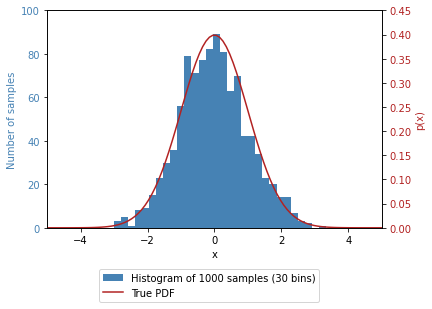
\includegraphics[width=\textwidth]{figures/gaussian_histogram_and_pdf.png}
        \caption{Gaussian distribution}
        \label{fig:gaussian_histogram_and_pdf}
    \end{subfigure}
    \hfill
    \begin{subfigure}[b]{0.45\textwidth}
        \centering
        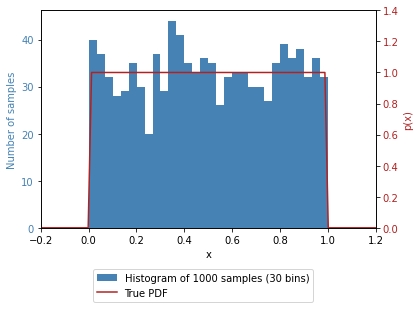
\includegraphics[width=\textwidth]{figures/uniform_histogram_and_pdf.png}
        \caption{Uniform distribution}
        \label{fig:uniform_histogram_and_pdf}
    \end{subfigure}
    \caption{Histogram of samples drawn from a distribution and true probability density function of distribution}
    \label{fig:histogram_and_pdf}
\end{figure}

%%%%%%%%%%%%%%%%%%%%%%%%%%

\subsection{Kernel density smoothing}

A smooth estimate of the probability density function is calculated using the kernel smoothing method with a Gaussian
kernel $\mathcal{N}(0, 1)$. The result is plotted for Gaussian and Uniform distributions in \autoref{fig:kernel_smoothed}.

\begin{figure}
    \centering
    \begin{subfigure}[b]{0.45\textwidth}
        \centering
        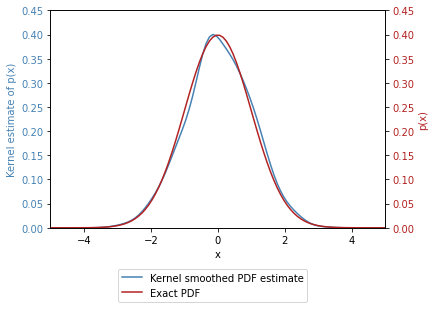
\includegraphics[width=\textwidth]{figures/gaussian_kernel_smoothed.png}
        \caption{Gaussian distribution}
        \label{fig:gaussian_kernel_smoothed}
    \end{subfigure}
    \hfill
    \begin{subfigure}[b]{0.45\textwidth}
        \centering
        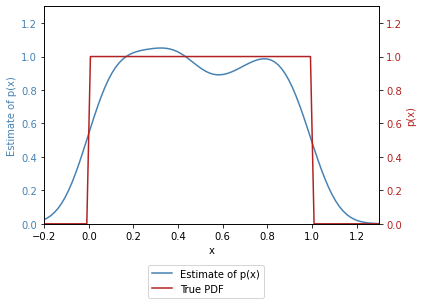
\includegraphics[width=\textwidth]{figures/uniform_kernel_smoothed.png}
        \caption{Uniform distribution}
        \label{fig:uniform_kernel_smoothed}
    \end{subfigure}
    \caption{Plot of true PDF and estimate of PDF generated using Gaussian kernel smoothing}
    \label{fig:kernel_smoothed}
\end{figure}

The kernel method takes an average of neighbouring values, weighted using a Gaussian distribution. This is advantageous
as it can smooth random irregularities in the samples: there may be histogram bins with a disproportionately high sample
count, which would give an incorrectly high estimate of the probability of this bin; the kernel smooths out this local
peak by taking neighbouring values into account. However, this also means that the kernel smoothing method becomes
inaccurate when there is a sudden change or discontinuity in the probability density function. In the Uniform
distribution there is zero probability for values outside the range $0<x<1$, but as the kernel averages over a window of
values it does not capture the step change at $x=0$ and $x=1$ and instead decays smoothly.

%%%%%%%%%%%%%%%%%%%%%%%%%%

\subsection{Multinomial distribution theory}

For N samples, let B be the random variable representing the number of samples in bin j. Let the probability that a
sample falls in bin j be $p_j$. By definition, the expected number of samples in bin j $\mu_j = \mathbb{E}[B] = N p_j$,
and the variance in the number of samples in bin j $\sigma^2_j = Var[B] = N p_j (1 - p_j)$.

For the Uniform distribution between 0 and 1, the pdf $p(x)$ is defined as:
\begin{align*}
    p(x) &= \frac{1}{x_{max} - x_{min}} \\
         &= 1
\end{align*}
Hence:
\begin{align*}
    p_j &= \int_{c_j - \delta/2}^{c_j + \delta/2}\,dx \\
        &= \delta \\
    \mu_j &= N \delta \\
    \sigma_j &= \sqrt{N \delta (1 - \delta)}
\end{align*}

In the histograms plotted in \autoref{},



%%%%%%%%%%%%%%%%%%%%%%%%%%
%%%%%%%%%%%%%%%%%%%%%%%%%%

\section{Conclusions}
\label{sec:conclusions}


%%%%%%%%%%%%%%%%%%%%%%%%%%
%%%%%%%%%%%%%%%%%%%%%%%%%%

% \begin{thebibliography}{9}
% \bibitem{}

% \end{thebibliography}


\end{document}